\chapter{Non-Orthogonal Multiple Access\\ (Invited Paper)}

\begin{center}
{\large\uppercase{Sanjeev Gurugopinath}} 

\vskip -6pt

Department of Electronics and Communication Engineering\\ 
PES University, Bengaluru 560085, India.
\end{center}

\newpage

\begin{multicols}{2}

\section*{Abstract}

Non-orthogonal multiple access (NOMA) has been recently proposed as a technique to increase the network throughput and to support massive connectivity, which are major requirements in the fifth generation (5G) communication systems. The NOMA can be realized through two different approaches, namely, in (a) power-domain, and (b) code-domain. In the power-domain NOMA (PD-NOMA), multiple users are assigned different power levels -- based on their individual channel quality information -- over the same orthogonal resources. The functionality of PD-NOMA comprises of two main techniques, namely, superposition coding at the transmitter and successive interference cancellation (SIC) at the receiver. An efficient implementation of SIC would facilitate to remove interference across the users. The SIC is carried out at users with the best channel conditions and is performed in descending order of the channel. On the other hand, in the code-domain NOMA (CD-NOMA), multiplexing is carried out using low-density spreading sequences for each user, similar to the code division multiple access (CDMA) technology. In this article, we provide an introduction to NOMA and present the details on the working principle of NOMA systems. Later, we discuss the different types of NOMA schemes under PD- and CD-domains, and investigate the related applications in the context of 5G communication systems. Additionally, we discuss the integration of NOMA with other technologies related to 5G such as cognitive radio and massive MIMO, and discuss some future research challenges.



\textit{Index Terms}---Fifth generation (5G) communication systems, interference mitigation, non-orthogonal multiple access (NOMA), successive interference cancellation (SIC), superposition coding (SC).


\section{Wireless Communication Systems}

The success story of the wireless communication technology is unprecedented. No other technology -- neither the radio, television nor personal computers; not even the internet -- has managed to attract billions of users in such a short time. Ever since the development of the first analog wireless communication system in the 1980s, a new generation of mobile communication system has been introduced in every decade. Each generation has received a considerable research attention in terms of the key innovations, wireless service, regulations and standards, from both the academia and the industry. The term \emph{innovations} refers to the factors related to the underlying technology, while the term \emph{service} represents the fundamental applications driving a particular generation -- such as voice calling, messaging service, internet, etc.

In the following, we provide a brief overview on each generation of the mobile communication systems, in terms of innovations, services and standards.

\subsection{First Generation (1G)} \label{SubSec_1G}

The spectrum during 1G was given free of cost to state-owned operators, and the user equipment, subscription, and the tariff were much higher as compared to the most expensive handsets and calling costs today. The basic service offered was high quality voice calling with excellent network coverage. Additionally, data communication such as facsimile was possible. The wireless standard used in the US was the advanced mobile phone system (AMPS); the Nordic mobile radio (NMR) system was used in most of European countries, and C-network -- which marked the start of the subscriber identity module (SIM) -- was used in Germany. The cellular handover across the European countries was not possible.

\subsection{Second Generation (2G)} \label{SubSec_2G}

The \emph{groupe speciale mobile} (GSM) was the dominant standard in 2G, which quickly gained worldwide popularity in the early 1990s. The other contemporary systems such as the IS-95 (in the US), and the Japanese personal digital (JPD) were proved to be no match to the growth of GSM. The monopoly of earlier operators was broken, which attracted competition from several operators in each country. This new regulation and the resulting competition is often credited for the massive success of GSM. Apart from voice calls, the short messaging system (SMS) was introduced; which not only became hugely popular, but also paved way for modern chatting applications such as WhatsApp. Digital data services were first introduced in GSM with a speed of $9.2$ kbps, which was further enhanced to tens of kbps to few hundreds of kbps through the general packet radio service (GPRS) and enhanced data rates for GSM evolution (EDGE) technologies, respectively. In terms of innovations, the user equipment became smaller and lighter for good, with extended battery lifetime lasting upto a few hours.

\subsection{Third Generation (3G)} \label{SubSec_3G}

The 3G era introduced the spectrum allotment via an open-market auction in some European countries such as the UK and Germany. Despite the high quoted prices, a few licenses were successfully auctioned. Subsequently, cellphones following the universal mobile telecommunication system (UMTS) were introduced. The selling point of UMTS was a high data rate of about $2$ Mbps. The initial models of UMTS phones were bulky with low battery life and attracted very less user attention, until phones comparable to the GSM-type models were manufactured. The auction-based regulation and the non user-friendly mobile phones were among several reasons which led to several industries filing bankruptcy and quitting the cellular business. The UMTS has largely turned out to be a superhype, and is proved to be a failure. Additionally, UMTS also faced a severe competition from the wireless local area network (WLAN) technology, which provided good connectivity with high data rates for a cheaper price.

\subsection{Fourth Generation (4G)} \label{SubSec_4G}

The failure of UMTS and success of WLAN led to the introduction of the long term evolution (LTE) in 4G, which is essentially a cleverly modified version of WLAN. Additionally, the operators got the spectrum licenses for significantly less money. The simultaneously introduced elimination of roaming charges for services such as voice calling, SMS and data across the  countries in parts of Europe and Asia helped in the success of LTE. The maximum speed promised by LTE is about $300$ Mbps in downlink and $50$ Mbps in uplink. Apart from the usual voice and data services, a technology similar to the voice over IP termed as the voice over LTE (VoLTE) has seen improved speech codec rates and voice quality. Currently, LTE is being improved with technologies such as massive multiple-input, multiple-output (MIMO) systems and device-to-device (D2D) communications.

\subsection{Fifth Generation (5G)} \label{SubSec_5G}

The 5G systems are envisioned to start functioning from 2020 onwards, with several promises such as significant improvements in data rates (about $10-20$ Gbps), latency (about $1$ ms), and spectral efficiency, as compared to LTE. Additionally, D2D and machine-to-machine (M2M) communications leading to the successful implementation of internet-of-things (IoT) is expected to be a reality very soon. The services offered in 5G are expected to find applications across various scenarios including vehicular networks, e-health, education, and industrial IoT. Some of the key innovations that drive 5G include massive MIMO, cognitive radios, millimeter wave communications, network virtualization, and software defined networking, to name a few. Although research surrounding 5G seems promising and exciting, several stake holders believe that 5G is superhyped, similar to the UMTS during 3G era. The services and promises surrounding 5G are strikingly similar to what was envisioned during 3G era, which includes applications in vehicular networks and IoT. However, the debate on whether this claim is true, and if not, how should the technologies driving 5G are expected to compete against LTE and LTE advanced are relevant topics of discussion for another study.

A summary of key comparative aspects in 1G -- 4G technologies are provided in Table~\ref{Tab_AllG}. One of the ``revolutionary'' features in the above mentioned generation of wireless communications are their respective multiple access techniques. The multiple access technologies used in 1G, 2G, 3G and 4G are frequency division multiple access (FDMA), time division multiple access (TDMA), code division multiple access (CDMA) and orthogonal frequency division multiple access (OFDMA), respectively. In the next section, we provide a brief description of these techniques.
\end{multicols} 

\begin{table}[ht]
\begin{center}
{\fontsize{8pt}{10pt}\selectfont
\caption{Comparison of 1G, 2G, 3G and 4G technologies.} \label{Tab_AllG}
\smallskip
\tabcolsep=4pt
\renewcommand{\arraystretch}{1.1}
\begin{tabular}{|c|c|c|c|c|}
\hline
\textbf{Parameters}              & \textbf{1G}                & \textbf{2G}                                 & \textbf{3G}                                   & \textbf{4G}                                                   \\ \hline
Year                    & 1980s             & 1993                               & 2001                                 & 2009                                                 \\ \hline
First Commercialization & USA               & Finland                            & Japan                                & South Korea                                          \\ \hline
Technology              & AMPS, NMT   & IS95, GSM                          & IMT2000, WCDMA                       & LTE, WiMax                                           \\ \hline
Multiple Access         & FDMA              & TDMA                               & CDMA                                 & OFDMA                                                \\ \hline
Switching               & Circuit Switching & Circuit/Packet Switching           & Packet Switching                     & Packet Switching                                     \\ \hline
Data Rates              & 2.4 -- 14.4 kbps  & 14.4 kbps                          & 3.1 Mbps                             & 100 Mbps                                             \\ \hline
Special Characteristics & First Wireless    & Digitalized 1G                     & Broadband                            & All IP, high speed                                   \\ \hline
Features                & Voice calls       & Multiple users voice calls         & Multimedia                           & Live streaming                                       \\ \hline
Supports                & Voice             & Voice and Data                     & Voice and Data                       & Voice and Data                                       \\ \hline
Internet Services       & Nil               & Narrowband                         & Broadband                            & Ultra Broadband                                      \\ \hline
Bandwidth               & Analog            & 25 MHz                             & 25 MHz                               & 100 MHz                                              \\ \hline
Operating Frequencies   & 800 MHz           & 900/1800 MHz                       & 2100 MHz                             & 850.1800 MHz                                         \\ \hline
Band Type               & Narrowband        & Narrowband                         & Wideband                             & Ultra Wideband                                       \\ \hline
Carrier Frequency       & 30 kHz            & 200 kHz                            & 5 MHz                                & 15 MHz                                               \\ \hline
Advantages              & Simple            & SMS/MMS, Internet access           & High security, Roaming & Speed, MIMO, Global mobility                         \\ \hline
Disadvantages           & Limited capacity  & Limited network range              & High power consumption               & Hardware complexity                                  \\ \hline
Applications            & Voice calls       & Voice calls, SMS, Browsing & Video conference, mobile TV     & High speed applications \\ \hline
\end{tabular}}\relax
\end{center}
\end{table}

\setcounter{figure}{0}
\begin{figure}
 \begin{center}
  \includegraphics[scale=0.75]{src/Figures/chap5/MultipleAccess.eps}
  \caption{Schematic representation of FDMA, TDMA and CDMA, used in 1G, 2G and 3G, respectively.} \label{Fig_MA}
 \end{center}
\end{figure}

\begin{multicols}{2}
\section{Orthogonal Multiple Access (OMA)} \label{Sec_OMA}
From the theoretical and design principle point of view, the TDMA, FDMA, CDMA and OFDMA belong to the class of orthogonal multiple access (OMA) techniques. The techniques in OMA all share a set of \emph{resources} across users, which are orthogonal to each other. This enables successful separation of information-bearing signals intended for each user, by employing optimal, low-complexity and cost-efficient receiver structures. These orthogonal resources are time, frequency, code and sub-carriers in case of TDMA, FDMA, CDMA and OFDMA, respectively. Next, we provide a brief explanation on all these schemes, in the light of earlier generation of mobile communication systems. A schematic representation of FDMA, TDMA and CDMA is shown in Figure~\ref{Fig_MA}.

\subsection{Frequency Division Multiple\hfill\break Access}
In FDMA, each user is allocated different bandwidths, which are wide enough to carry the information-bearing signal spectrum. This OMA technique was widely used in classical wired telephone systems and subsequently in the 1G analog wireless systems. Other than that, FDMA is also used in digital TV cable television, fiber optics, and aerospace telemetry. Early satellite systems also used FDMA.

\subsection{Time Division Multiple Access}
The TDMA was an integral part of the 2G communication system, and is used by the celebrated GSM technology. In TDMA, every channel/bandwidth is divided into time slots and each user sends its information over different time slots, sequentially. Ideal for the relatively slowly varying voice signals -- the backbone of GSM, the TDMA finds less utility in transmission of high-speed data. In GSM, the spectrum is divided into eight time slots of 200 kHz band each, where each slot is transmitted at a rate of 270 kbps using the Gaussian minimum shift keying (GMSK) modulation.

\subsection{Code Division Multiple Access}
One of the earliest forms of the direct sequence spread spectrum technique, CDMA spreads the data over the entire bandwidth with a lower power level. The CDMA is the dominant multiple access technology in 3G communication systems. Each user is assigned a sequence of spreading codes, which are orthonormal with each other. This technique enables the users to use the entire available bandwidth at the same time, without inter-user interference. In the IS-95 standard, CDMA is used with a digitally compressed voice at 13 kbps, which is spread using a 1.2288 Mbps chip sequence derived from a pseudo random code generator. As a result, the voice signal is spread over a bandwidth of 1.25 MHz. At the receiver, correlator circuit is used to separate out the intended signal from the rest. The wideband CDMA (W-CDMA) uses CDMA with 3.84 Mbps chip sequences over a 5 MHz wideband channel.

\subsection{Orthogonal Frequency Division Multiple Access}
The dominant multiple access technology in LTE for 4G communication systems, OFDMA uses a multi-carrier modulation technique to divide a wideband channel into several narrowband channels, where the employed subcarriers are orthogonal to each other. In LTE, each band is divided into 15 kHz wide subcarriers. The data to be transmitted is divided into bit streams with lower speed, which are modulated onto the subcarriers. Apart from being spectrally efficient, the OFDMA also offers high data rates and a better resilience to frequency selective fading. In LTE, the smallest group of allotted subchannels is called as a \emph{resource block} (RB). Each user is allotted a number of RBs, depending on the requirement.

In the following, we use a common terminology to the orthogonal entities in FDMA, TDMA, CDMA and OFDMA, namely, frequency, time, code and subcarriers collectively as \emph{orthogonal resources}. In OMA, it is intuitive that the number of users that can be supported in a cell directly depends on the number of available orthogonal resources. Moreover, although the theoretical development in OMA predicts that a low-complexity receiver structure suffices, the practical implementation part has a different story to tell. The largely time-varying statistical nature of the wireless channel adds significant impairment to the information-bearing signals intended for each users, and destroys a part of their orthogonality. Restoring of orthogonality requires more complicated methods at the receiver.

Low-complexity receivers and accommodation of massive number of users in a cell are an integral part of the 5G vision. Towards this end, the non-orthogonal multiple access (NOMA) techniques are envisioned as a promising solution \cite{Chen_ComMag_2018}. In the following, we describe the principle of NOMA and discuss different NOMA techniques. As a summary, Figure~\ref{Fig_OMAandNOMA} shows the types and milestones of the orthogonal and non-orthogonal multiple access techniques.

\section{Non-Orthogonal Multiple Access (NOMA)}  \label{SecNOMA}
In the following, we present the working principle of NOMA, provide a performance comparison with that of OMA and discuss its advantages over OMA. The main idea behind NOMA is to overcome the limited user capacity in OMA, that is, to support more users than the available orthogonal resources \cite{Dai_ComMag_2015}. Thus, the resource allocation across users become ``non-orthogonal'', and the support of extra set of users comes at the cost of an increase in the receiver complexity \cite{Yuan_ComMag_2016}.

The non-orthogonality of resources in NOMA brings in an additional challenge of inter-user interference and hence the need for a scheme to eliminate this interference arises, which increases the receiver complexity by atleast a polynomial order \cite{Ding_ComMag_2017}. Historically, NOMA was proposed as an interference mitigation technique in CDMA systems, where a number of non-orthogonal sequences more than the number of chips was needed to support more number of users. Broadly speaking, the NOMA schemes can be divided into the following two categories \cite{Dai_CST_2018}. More details on the technical-front are provided in the next section.
\end{multicols}


\begin{figure}[ht]
\begin{center}
 \includegraphics[scale=0.75]{src/Figures/chap5/NOMA_AllTechnologies.eps}
 \caption{Types and milestones of multiple access technologies.} \label{Fig_OMAandNOMA}
\end{center}
\end{figure}

\begin{multicols}{2}
\begin{enumerate}
 \item[I.] \underline{Power-domain NOMA}: In this scheme, different power levels are allocated to different users, depending on the quality of their respective channels. That is, different users are serviced over the same orthogonal resource (time, frequency or code), but with different power levels. At the user end, the difference in the power level is exploited by using the \emph{successive interference cancellation} technique. Broadly speaking, each user decodes the signals of other users and removes them before decoding its own signal, depending on its allocated power.
 \item[II.] \underline{Code-domain NOMA}: The working of code-domain NOMA is similar to that of CDMA, except that the codes used are either low-density or non-orthogonal with a low cross-correlation value.
\end{enumerate}

\section{Types of NOMA Schemes} \label{SecNOMA_Types}
In this section, we first present the power-domain NOMA (PD-NOMA) and discuss the key schemes in PD-NOMA, namely, the superposition coding at the transmitter and the successive interference cancellation at the receiver. Next, we discuss the non-orthogonality in the code domain through code-domain NOMA (CD-NOMA) and discuss different schemes in CD-NOMA.

\subsection{Power-Domain NOMA} \label{SubSecPDNOMA}
The PD-NOMA can be visualized as a multiple access in a new domain, namely the power-domain, as opposed to other resource domains such as time, frequency or code. At the transmitter side, different information-bearing signals corresponding to different users are superimposed on each other with different power levels, over a single resource block, that is, over the same time, same frequency or with the same code. At the receiver, mutli-user detection schemes such as the successive interference cancellation is used to separate the signals.

\smallskip

\noindent
{\bf Superposition Coding}
\smallskip

For clarity, let us consider a cellular network with one base station (BS) and two users $U_1$ and $U_2$ as shown in Figure~\ref{Fig-SC2Users}. The signal sent to each user suffers from fading and path loss, which is directly dependent on the distance between each user and the BS. As shown in Figure~\ref{Fig-SC2Users}, let us assume that $U_1$ is far-away from the BS and $U_2$ is closer to the BS. In this way, the channel quality from BS to $U_1$ will be inferior/degraded as compared to the channel quality from the BS to $U_2$. In other words, the average received signal-to-noise (SNR) at $U_1$ will be less compared to the average SNR at $U_2$. Let the signals correspond to $U_1$ and $U_2$ be $y_1$ and $y_2$, and $P$ be the average power available at the BS. The BS transmits
\setcounter{equation}{0}
\begin{align}
z = \sqrt{\zeta P} y_1 + \sqrt{(1-\zeta) P} y_2,
\end{align}
where $0 < \zeta < 1$ is the fractional power allocation factor for $U_1$. Since the power allocation coefficient is inversely proportional to the average SNR, power given to $U_1$ will be larger than $U_2$, that is $\zeta > 0.5$. The superimposed signal $z$ is transmitted to $U_1$ and $U_2$ simultaneously over the same resource block.
\begin{figure}[H]
\centering
  \includegraphics[scale=0.5]{src/Figures/chap5/NOMA_SC_2Users.eps}
  \caption{Comparison of OMA and PD-NOMA with superposition coding.} \label{Fig-SC2Users}
\end{figure}
The above principle can be extended to $N > 2$ users as follows. The users are ordered based on their channel quality, and their power level is decided accordingly. Without loss of generality, let the users $U_1, U_2, \ldots, U_N$ be ordered according to the descending order of their distances from the BS. Let $\zeta_i, i=1,\ldots,N$ denote the power allocation coefficient to each user, respectively. Therefore, the signal transmitted by the BS is given as
\begin{align}
z = \sqrt{\zeta_i P} y_i,
\end{align}
where $y_i$ represents the signal corresponding to the $i^{\text{th}}$ user. The decoding of signals at each user is carried out through successive interference cancellation, which is described next.

\subsubsection{Successive Interference Cancellation}
The successive interference cancellation (SIC) is a type of multi-user detection technique, and an iterative procedure. Let us consider the 2 user example in Figure~\ref{Fig-SIC2Users}. Since $U_1$ is the far user -- with a lower average received SNR value and higher allocated power, it directly decodes its own signal $y_1$ by treating the interference due to $y_2$ as noise. On the other hand, $U_2$ being allocated lower power, first decodes $y_1$ and cancels it from its from the received superimposed signal before decoding its own signal, $y_2$.
\begin{figure}[H]
\centering
  \includegraphics[scale=0.49]{src/Figures/chap5/NOMA_SIC_2Users.eps}
  \caption{Successive interference cancellation procedure with 2 users.} \label{Fig-SIC2Users}
\vskip -.2cm
\end{figure}

This procedure can accordingly be extended the case of $N$ users. The user with the weakest channel, $U_1$, decodes its own signal by treating the interference due to other signals as noise. The $i^{\text{th}}$ user, $i \in \{2,\ldots,N\}$, first cancels the interference due to the $j^{\text{th}}$ user, $j \leq i-1$, and canceling it before decoding its own signal. As an example, the case of 3 users is illustrated in Figure~\ref{Fig-SIC3Users}. $U_1$ directly decodes its own signal, and $U_2$ decodes the signal of $U_1$ first and cancels it before decoding its own signal. Likewise, $U_3$ first decodes the signal of $U_1$, cancels it, then decodes the signal of $U_2$ and cancels it before decoding its own signal.
\begin{figure}[H]
\centering
  \includegraphics[scale=0.47]{src/Figures/chap5/NOMA_SIC_3Users.eps}
  \caption{Successive interference cancellation procedure with 3 users.} \label{Fig-SIC3Users}
\vskip -.2cm
\end{figure}

As mentioned earlier, NOMA achieves the average capacity in both downlink and uplink AWGN channels. However, when the number of users sharing a particular orthogonal resource is high, the error propagation due to SIC might degrade the performance in terms of bit error probability. 

\smallskip
\noindent
{\bf Application of PD-NOMA}


As an application, the PD-NOMA has been employed successfully in the ATSC 3.0 digital TV broadcasting standard in the US. The technology is termed as the layered division multiplexing (LDM), and works a follows. The ATSC 3.0 standard encourages the usage of a two-layer power domain multiplexed signal, divided as the upper layer (UL) and the lower layer (LL). The LL is intended for high data rate, high definition digital TV service, while the UL is allotted a higher power and is intended for portable devices with lower data rates. At the user end, the UL signal is directly decoded while treating the interference due to LL signal as noise -- thereby losing a small fraction of the data rate, and the LL signal is decoded through SIC procedure. It has been observed that the LDM has a better performance in comparison with the regular FDMA, which increases directly with the received SNR at the fixed TV unit.\\[-.5cm]

\subsection{Code-Domain NOMA} \label{SubSecCDNOMA}

We now turn our attention to the code-domain NOMA (CD-NOMA). As mentioned earlier, the key aspect of the CD-NOMA finds its roots in CDMA, where users share the same time-frequency resources and are multiplexed by orthogonal codes. More users can be accommodated by introducing low cross-correlation sequences. In what follows, we provide brief explanation on different types of CD-NOMA.

\smallskip
\noindent
{\bf Low-Density Spreading CDMA}


The low-density spreading CDMA (LDS-CDMA) was the first method conceived from CDMA, where low-density spreading instead of conventional spreading sequences. It has been shown that under certain conditions, LDS-CDMA achieves the single-user performance. At the transmitter, the symbols are modulated into sparse spreading sequences -- that is, the number of non-zero elements in the spreading sequence is lower than the number of chips -- as opposed to the ``fully-populated'' sequences. Therefore, the number of superimposed signals at each chip will be less than the number of users. This helps in interference mitigation, and the key design factor includes the choice of spreading sequences. At the receiver, the decoding is based on the optimal maximum likelihood technique, which is computationally complex. Message passing technique-based multi-user detection strategies have been proposed as a class of low complexity alternatives.

\smallskip
\noindent
{\bf Low-Density Spreading OFDM}

The multi-carrier version of CDMA, called as the multi-carrier CDMA (MC-CDMA) is closely related to OFDM. The idea of LDS-CDMA has been extended to OFDM, resulting in LDS-OFDM. Recall that in conventional OFDM systems, a message symbol is mapped to a specific subcarrier and the design is such that the subcarriers are orthogonal. On the other hand, in LDS-OFDM, the symbols are multiplexed using the LDS sequences and the chips are carried on different subcarriers. It is observed that the performance of LDS-OFDM is resilient to frequency-selective fading, in comparison with the performance of LDS-CDMA.

\smallskip
\noindent
{\bf Sparse Code Multiple Access}

Sparse code multiple access (SCMA) is a relatively newly introduced CD-NOMA technique. The theory behind SCMA is slightly involved. Broadly speaking, instead of two separate steps of mapping the raw bits to a constellation point followed by spreading, the bits are directly mapped to sparse coded sequences. Each user uses its own codebook for this mapping. Design of the maximum number of such codebooks is of primary importance. All codewords in a codebook are sparse along a particular dimension, and makes the codewords across codebooks as unique, so as to avoid the interference between users. At the receiver, techniques such as message passing algorithms can be used for decoding the bits. The performance of SCMA has been observed with real-time prototyping, and the results indicate that the number of users can be increased upto three-fold more than the number of orthogonal resources, while maintaining error-levels close to that of OMA.

\smallskip
\noindent
{\bf Multi-User Shared Access}

The multi-user shared access (MUSA) requires a set of low cross-correlation spreading sequences. Although not a strict requirement, MUSA based on the sparse spreading sequences can also be designed. In the uplink, the transmitted symbols of a particular user are spread using the same spreading sequence. Then, these symbols are transmitted over the same orthogonal resource -- typically, OFDM. At the receiver, a combination of linear processing and SIC are used to separate the symbols from each user. On the other hand, in the downlink of MUSA, users are grouped together. In each group, the symbols corresponding to each user is allotted different power levels and are superimposed. The spreading sequences chosen per group are same across all the users in that group, while the sequences are orthogonal across groups. In this way, SIC can be employed at the users to decode their own symbol.

\smallskip
\noindent
{\bf SIC-Aided Multiple Access}

The working principle of SIC-aided multiple access (SAMA) is similar to that of MUSA, except that the non-zero entries in the codewords across all users is set to unity. The framework is assumed to be sparse, that is, the number of users are larger than the number of subcarriers in OFDM. In SAMA, the linear transformation that carries out the spreading follows the two requirements. First, the number of groups with different number of non-zero elements in a spreading sequence should be as high as possible. Secondly, the number of overlapped spreading sequences which have the same number of non-zero elements should be as low as possible. Based on such a design, it can be shown that if $N$ is the number of OFDM subcarriers, then the maximum number of users can be shown to be $2^N-1$. At the receiver, message passing algorithm is employed to decode the symbol of each user.

\subsection{Other NOMA Schemes}
Several other NOMA schemes other than the PD-NOMA and CD-NOMA have also been proposed in the literature. We provide a brief discussion on some of these techniques in the following.

\smallskip
\noindent
{\bf Spatial Division Multiple Access}


As mentioned earlier, even though orthogonal codes are used in CDMA, the orthogonality is typically affected due to the convolution with the channel impulse response. Towards this end, one solution could be to use sequences based on user-specific channel impulse response rather than plain orthogonal sequences, which is referred to as the spatial division multiple access (SDMA). On the good side, this scheme allows massive number of users to be served, with a performance similar to other CD-NOMA techniques. However, the practical applicability of this technique is questionable, since they require accurate estimation of the respective channel impulse responses. Towards this end, the SDMA requires of high computational iterative algorithms such as particle swarm optimization, genetic algorithms, or other machine learning-based techniques. 

\smallskip
\noindent
{\bf Pattern Division Multiple Access}


In the pattern division multiple access (PDMA), employs non-orthogonal patterns, which are designed by jointly optimizing the achievable diversity and correlation across the users. These patterns are, as usual, multiplexed over orthogonal resources. Employing the code-domain for multiplexing gives SAMA, and employing the spatial domain yields a technique called as spatial PDMA. It has been observed that spatial PDMA offers a better performance as compared to multi-user MIMO, without an additional burden of design of a precoder.


\eject

\smallskip
\noindent
{\bf Signature-Based NOMA}


Low code rate and signature-based shared access (LSSA) is one of the types of a signature-based NOMA (SNOMA) techniques proposed for uplink massive machine-type communications, where each user data is multiplexed at the bit level by employing a specific signature pattern. Another technique in SNOMA is called the resource spread multiple access (RSMA), which assigns unique signature patterns to each user before spreading the signal over the available resource. Both LSSA and RSMA have single- and mutli-carrier variants, for advantages such as low power consumption and low latency.

\smallskip
\noindent
{\bf Interleave-Based NOMA}


The interleave division multiple access (IDMA) is a type of interleave-based NOMA, where the chips after spreading are interleaved before transmission. In other words, IDMA is CDMA with interleaved chips. It has been reported that the IDMA is capable of achieving a better BER as compared to CDMA, which is due to the fact that interleaving on chips results in a better diversity gain as compared to the conventional bit interleaving. Another related technique is the interleave-grid multiple access (IGMA), where the users are distinguished based on their bit-interleaving patterns, grid mapping patterns or a combination of both. The IGMA is capable of mitigating the performance degradation due to frequency selective fading and inter-cell interference. The decoding complexity is also tolerable, and can be improved further by exploiting a sparse grid mapping pattern.

\smallskip
\noindent
{\bf Spreading-Based NOMA}


There exists several techniques for NOMA based on spreading codes, with non-orthogonal coded multiple access (NCMA) being one of them. The basic principle of NCMA is to exploit non-orthogonal spreading codes with low correlation for resource spreading. The NCMA receiver exploits the parallel interference cancellation (PIC), whose computational complexity is lower than SIC. Non-orthogonal coded access (NOCA) is another spreading-based NOMA, where the symbols are spread using non-orthogonal sequences, before transmission.

\smallskip
\noindent
{\bf Bit Division Multiplexing}


In bit division multiplexing (BDM), the resource allocation across users happens at the bit level and not at the symbol level. Although the resource allocation in BDM is orthogonal in the bit domain, the bits can be superimposed in the symbol domain since the users can share the same constellation.

\bigskip
\noindent
{\bf Compressive Sensing-Based NOMA}


Compressive sensing (CS) is a relatively new research topic, where a sparse signal (or a signal which can be represented sparsely in a vector space) can be sampled well-below the Nyquist rate and can be reconstructed correctly with overwhelming probability by employing optimization techniques that are solvable in polynomial time. A class of CS-based NOMA techniques have been proposed recently, such as the class of asynchronous random access protocols. Given that sparse nature of the signals represents in several NOMA schemes studied above, CS is expected to play a crucial role in practical realization of NOMA schemes for 5G.

\smallskip
\noindent
{\bf Miscellaneous Schemes}

Several other industries has also placed a vital role in developing several NOMA techniques, as a part of the release 14 3GPP NR Study Item. Among these, the low density spreading signature vector extension (LDS-SVE) was proposed by Fujitsu. Intel proposed the frequency domain spreading (FDS) and low code rate spreading (LCRS). The LDS-SVE, FDS and LCRS can be categorized under the spreading-based NOMA class. Another interleaver-based NOMA scheme called as the repetition division multiple access (RDMA) was proposed by MTK. The RDMA is capable of separating user symbols multiplexed over same orthogonal resources, by exploiting the cyclic shift repetition of the modulated symbols.

A summary of the NOMA schemes proposed for release 14 3GPP NR Study Item is provided in Table~\ref{Tab_3GPP}
\begin{table}[H]
\centering
\caption{NOMA schemes in release 14 3GPP NR Study Item.} \label{Tab_3GPP}
\medskip
\renewcommand{\arraystretch}{1.17}
\begin{tabular}{|c|c|c|}
\hline
\textbf{NOMA}    & \textbf{Industry} & \textbf{Uplink / Downlink} \\ \hline
PD-NOMA \cite{Benjebbour_CSCN_2015} & DCM      & UL / DL           \\ \hline
SCMA \cite{Nikopour_PIMRC_2013}    & Huawei   & UL / DL           \\ \hline
MUSA \cite{Yuan_VTC_2016}   & ZTE      & UL / DL           \\ \hline
PDMA \cite{Dai_WC_2018}    & CATT     & UL / DL           \\ \hline
LSSA    & ETRI     & UL                \\ \hline
RSMA    & Qualcomm & UL                \\ \hline
IGMA    & Samsung  & UL / DL           \\ \hline
IDMA \cite{Kusume_TWC_2012}    & Nokia    & UL                \\ \hline
NCMA    & LGE      & UL                \\ \hline
NOCA    & Nokia    & UL                \\ \hline
GOCA    & MTK      & UL                \\ \hline
LDS-SVE & Fujitsu  & UL / DL           \\ \hline
FDS     & Intel    & UL                \\ \hline
LCRS    & Intel    & UL                \\ \hline
RDMA    & MTK      & UL                \\ \hline
\end{tabular}
\end{table}


\section{Performance and Comparison\hfill\break with OMA} \label{SecNOMAOMA}
It was mentioned earlier that a combination of SC at the transmitter and SIC at the receiver is used in PD-NOMA. This choice of the SC-SIC pair is due to a classic result in information theory. It is known that that SC-SIC strategy achieves the capacity region of the single-input single-output (SISO) broadcast channel impaired by additive white Gaussian noise. Additionally, it is also known that capacity region of the SC-SIC scheme is larger than that of any OMA scheme, when the users experience different channel strengths. However, when the channel strengths are similar, NOMA does not offer any performance benefit in terms of the achievable rate, as compared to OMA. Figure~\ref{Fig-RR}~ gives an illustration on the achievable rate regions of NOMA and OMA with symmetric and asymmetric channels, following the above discussion.
\begin{figure}[H]
 \centering
  \includegraphics[scale=0.63]{src/Figures/chap5/RateRegions.eps}
  \caption{Comparison of rate regions of downlink NOMA and OMA with symmetric (on the left) and asymmetric (on the right) channels. NOMA offers a better rate region when the channel strengths are different.} \label{Fig-RR}
\end{figure}

NOMA offers several advantages over OMA, and some of them are briefed below.
\begin{enumerate}
 \item Improved spectral efficiency -- The spectral efficiency achieved due to NOMA is higher than that of OMA in several scenarios, due to the above mentioned result in information theory on Gaussian broadcast channels.
 \item Enabling massive connectivity -- Enabling the use of non-orthogonal resources enhances the number of users served in a single cell, and is not dependent on the available number of orthogonal resources anymore. If the users are equipped with high-computing receivers, NOMA possesses the capacity to support massive connectivity.
 \item Low latency in transmission -- In OMA systems, each user has to first send a scheduling request in the uplink, and the base station responds to it by sending out a clear-to-send signal before starting service. This introduces high latency, which can be a bottleneck in massively connected 5G systems. On the contrary, grant-free multiple access is possible in uplink NOMA. In other words, grant-free access on uplink can be achieved for users associated with pre-configured resources in a resource-domain. More details on this aspect will be provided in Section~\ref{SecNOMA_Types}
 \item Limited channel feedback -- Specifically in the power-domain NOMA, the requirement on the feedback of the channel state information (CSI) is relaxed, because an accurate knowledge of CSI is only required during power allocation for users. 
\end{enumerate}

\section{Integration of NOMA with Other\\5G-Related Technologies}
In this section, we discuss the utility of NOMA with some of the other technologies envisioned to be an integral part of 5G communication networks. In each case, we argue that performance enhancement is achievable due to NOMA.

\subsection{Cognitive Radio}
Cognitive radios (CR) are expected to be capable of intelligently find the vacant spectra over a wide bandwidth, which are unused by the respective licensed users over time, frequency and space to opportunistically utilize the available spectrum for its own communication. The CR terminates its communication when the licensed user intends to use the spectrum. There are several ways in which the NOMA technique can be integrated with CR technology \cite{Lv_ComMag_2018}, \cite{Yu_Access_2019}. The procedure to find whether a licensed spectrum is active or not is called as \emph{spectrum sensing}. Currently, most of the literature carrier out performance analysis of CR networks in terms of either spectral efficiency or energy efficiency, under imperfect sensing conditions. On the other hand, when the CR employs NOMA scheme to accommodate more uses when the licensed spectrum is found to be free, the spectral/energy efficiency can be greatly improved. From the CR communication perspective, the user with a weaker channel can be viewed as the licensed user, and hence a set of secondary/CR receivers can be accommodated when the licensed receiver has a low SNR. The overall network efficiency can be improved by allowing the performance degradation at the licensed user to be within allowable limits.

\subsection{Massive MIMO}
The spectral efficiency of a network employing NOMA can be further improved by employing more number of antennas at the transmitter and the receiver, by exploiting the spatial diversity/multiplexing gain. However, the design of MIMO-NOMA strategy is not simple. For example, consider the PD-NOMA for a MIMO system. The SC is employed at the transmitter for a single-input single-output (SISO) network, based on the user power levels, which are scalars. However, in case of MIMO, the channel matrix makes the task of assigning power allocation factors challenging. One of the possible solutions is to form multiple beams in the downlink, and the users oriented towards one beam can be served simultaneously using PD-NOMA. Another idea is to carry out beamforming to individual users, with the constraint on power allocation.

\subsection{Full Duplex Communication\\ Systems}
Full duplex (FD) communications enables simultaneous transmission and reception of signals on the same frequency band, and is envisioned as one of the key technologies to enhance spectral efficiency in 5G communication systems. A key factor affecting the performance of FD systems is the presence of self-interference (SI), and recent advances in transceiver and antenna design show a promising trend to cancel SI upto the receiver noise floor. The integration of FD and NOMA is interesting, and the idea is to enable simultaneous uplink and downlink transmission over a resource, carrying NOMA signal both ways \cite{Mohammadi_ComMag_2019}. However, integrating the two techniques is known to be a hard problem, since SI in an FD-NOMA system significantly affects its performance. Broadly speaking, each user requires to cancel its SI, before canceling the interference due to other users, while employing SIC. Therefore, interference management in FD-NOMA systems is an interesting research topic. Another approach where an FD-NOMA system can be employed is in where \emph{strong} NOMA users -- which acts as relays -- assist the transmissions between a base station and \emph{weak} NOMA users. In this case, security and reliability while maintaining the required low latency are the key issues to be considered. Given the complex receiver structure in FD-NOMA systems, machine learning and neural network-tuned encoding and decoding schemes can be useful in maximizing the network performance.

\subsection{Visible Light Communications\hfill\break and Free-Space Optics}
Spectrum scarcity in kHz/MHz/GHz range is one of the key issues in 5G communication systems, especially for applications such as IoT. Towards this end, high data rate-driven short range communications employing the visible light communications (VLC) or free space optics (FSO) has emerged as a promising small cell technology. The operating bandwidth of infrared unlicensed spectrum is 300 GHz -- 430 THz, while VLC operates in 430 THz -- 790 THz. A key advantage in VLC is the simplicity in transceiver design, which consists of off-the-shelf light emitting diodes (LED) and simple photodiodes. Additional advantages include its non-vulnerability to interference due to RF signals, and ensured safety in places such as hospitals. The combination of VLC/FSO and PD-NOMA results in the so-called optical NOMA (O-NOMA) \cite{Marshoud_WC_2018}, which is ideal to employ PD-NOMA because of the high SNR due to the presence of a overwhelmingly dominant line-of-sight component. A study on the performance of O-NOMA systems in terms of the achievable rate, BER, inter- and intra-cell interference and power allocation form are interesting and challenging. A major challenge in O-NOMA systems is in channel symmetry. It was mentioned earlier in Sec.~\ref{SecNOMAOMA} that channel asymmetry plays a primary role in the performance of NOMA in comparison with the performance of OMA. The short range and focused communication in VLC due to the presence of a line-of-sight creates a close channel symmetry between two users in the small cell. Other challenges include enabling MIMO-O-NOMA, design of uplink O-NOMA, effects of non-linearity due to LED and other circuitry and optimal user multiplexing using hybrid O-NOMA.

\section{Future Research Challenges}
In this section, we discuss some of the key areas of research related to NOMA. The existing NOMA schemes employ a single strategy for a variety of applications under the 5G umbrella such as cellular communication, wireless sensor networks, e-health, vehicular networks and internet-of-things, to name a few. The performance of a NOMA-aided system can be improved significantly by designing specific strategies for a particular application. Design and analysis of a software-defined NOMA system with flexible configuration is of significant interest. Additionally, specific challenges such as accurate feedback of channel quality information in SISO-NOMA, optimal beamforming design in MIMO-NOMA, cooperation among the base stations in coordinated multipoint (CoMP)-aided NOMA, PAPR reduction in LDS-NOMA and low cross-correlation spreading sequence design in CD-NOMA also need resolving.

Most of the analysis carried out in literature assumes a two-user PD-NOMA network, such as the case considered in the example depicted in Figure~\ref{Fig-SC2Users}. Although accommodating more users over a resource is possible theoretically, the SC-SIC scheme induces additional computational complexity, which increases significantly with an increase in the number of users. A solution to overcome this problem is to divide the network into number of clusters, with two or more users per cluster. Orthogonal resources are allotted for each cluster. However, dynamic allocation of users to form a cluster and deciding number of users per cluster is a fairly challenging problem. The resulting optimization problem is NP-hard and hence, finding a solution through exhaustive search is computationally not feasible. Towards this end, algorithms with low-complexity are required to enable quick network dynamics.

Another interesting area of research is in developing effective hybrid multiple access schemes. For the requirement of massive connectivity and efficient utilization of available resources in 5G networks, hybrid multiple schemes -- e.g., the combination of NOMA and OFDM -- can be considered. A study on how to combine NOMA with other OMA techniques can be useful, and game-theoretic formulations can be considered to optimize resources in the power/code and other orthogonal domains such as frequency/time/code \cite{Wang_TWC_2019}.

Apart from performance analysis of NOMA systems from purely a PHY layer perspective such as BER and channel capacity, cross-layer aspects in NOMA also play an important role to provide a generalized framework to cover diverse applications in 5G. Some of the performance measures for cross-layer optimization include spectral efficiency, energy efficiency, low latency and massive network connectivity. A study on the impact of efficient design of modulation and coding schemes in PHY layer on higher layers is important in NOMA, since NOMA also ensures user fairness along with quality-of-service (QoS). Problems such as user pairing and scheduling have to be jointly optimized along with requirements such as power allocation, channel estimation and re-transmission strategy design.

\section{Conclusion}
In this article, we have discussed the working principle, key advantages and performance benefits of the non-orthogonal multiple access (NOMA), which is recognized as one of the promising feature for 5G communication systems. Different types of NOMA systems, which can be largely classified under the power-domain NOMA (PD-NOMA) and code-domain NOMA (CD-NOMA) categories were discussed in terms of their methodology, key aspects, and receiver complexities. We also discussed the specific regimes where NOMA outperforms OMA, and detailed the potential integration of NOMA with other 5G-related technologies. Finally, we also briefed on the future research directions in NOMA. The NOMA is expected to play a vital role in supporting the implementation of 5G wireless communication systems with massive connectivity and low latency.

\begin{thebibliography}{99}
\bibitem{Chen_ComMag_2018}
Y.~{Chen}, A.~{Bayesteh}, Y.~{Wu}, B.~{Ren}, S.~{Kang}, S.~{Sun}, Q.~{Xiong},
  C.~{Qian}, B.~{Yu}, Z.~{Ding}, S.~{Wang}, S.~{Han}, X.~{Hou}, H.~{Lin},
  R.~{Visoz}, and R.~{Razavi}, ``Toward the standardization of non-orthogonal
  multiple access for next generation wireless networks,'' \emph{{IEEE} Commun.
  Mag.}, vol.~56, no.~3, pp. 19--27, Mar. 2018.

\bibitem{Dai_ComMag_2015}
L.~{Dai}, B.~{Wang}, Y.~{Yuan}, S.~{Han}, C.~{I}, and Z.~{Wang},
  ``Non-orthogonal multiple access for {5G}: {S}olutions, challenges,
  opportunities, and future research trends,'' \emph{{IEEE} Commun. Mag.},
  vol.~53, no.~9, pp. 74--81, Sep. 2015.

\bibitem{Yuan_ComMag_2016}
Y.~{Yuan}, Z.~{Yuan}, G.~{Yu}, C.~{Hwang}, P.~{Liao}, A.~{Li}, and K.~{Takeda},
  ``Non-orthogonal transmission technology in {LTE} evolution,'' \emph{{IEEE}
  Commun. Mag.}, vol.~54, no.~7, pp. 68--74, Jul. 2016.

\bibitem{Ding_ComMag_2017}
Z.~{Ding}, Y.~{Liu}, J.~{Choi}, Q.~{Sun}, M.~{Elkashlan}, C.~{I}, and H.~V.
  {Poor}, ``Application of non-orthogonal multiple access in {LTE} and {5G}
  networks,'' \emph{{IEEE} Commun. Mag.}, vol.~55, no.~2, pp. 185--191, Feb.
  2017.

\bibitem{Dai_CST_2018}
L.~{Dai}, B.~{Wang}, Z.~{Ding}, Z.~{Wang}, S.~{Chen}, and L.~{Hanzo}, ``A
  survey of non-orthogonal multiple access for {5G},'' \emph{{IEEE} Commun.
  Surveys Tuts.}, vol.~20, no.~3, pp. 2294--2323, Third Quarter 2018.

\bibitem{Benjebbour_CSCN_2015}
A.~{Benjebbour}, A.~{Li}, K.~{Saito}, Y.~{Saito}, Y.~{Kishiyama}, and
  T.~{Nakamura}, ``{NOMA}: {F}rom concept to standardization,'' in
  \emph{Proc.~2015 IEEE Conference on Standards for Communications and
  Networking {(CSCN)}}, Oct. 2015, pp. 18--23.

\bibitem{Nikopour_PIMRC_2013}
H.~{Nikopour} and H.~{Baligh}, ``Sparse code multiple access,'' in
  \emph{Proc.~2013 IEEE 24th Annual International Symposium on Personal,
  Indoor, and Mobile Radio Communications {(PIMRC)}}, Sep. 2013, pp. 332--336.

\bibitem{Yuan_VTC_2016}
Z.~{Yuan}, G.~{Yu}, W.~{Li}, Y.~{Yuan}, X.~{Wang}, and J.~{Xu}, ``Multi-user
  shared access for internet of things,'' in \emph{Proc.~2016 IEEE 83rd
  Vehicular Technology Conference ({VTC} Spring)}, May 2016, pp. 1--5.

\bibitem{Dai_WC_2018}
X.~{Dai}, Z.~{Zhang}, B.~{Bai}, S.~{Chen}, and S.~{Sun}, ``Pattern division
  multiple access: A new multiple access technology for 5g,'' \emph{{IEEE
  Wireless Commun.}}, vol.~25, no.~2, pp. 54--60, Apr. 2018.

\bibitem{Kusume_TWC_2012}
K.~{Kusume}, G.~{Bauch}, and W.~{Utschick}, ``{IDMA vs. CDMA}: {A}nalysis and
  comparison of two multiple access schemes,'' \emph{IEEE Trans.\ Wireless
  Commun.}, vol.~11, no.~1, pp. 78--87, Jan. 2012.

\bibitem{Lv_ComMag_2018}
L.~{Lv}, J.~{Chen}, Q.~{Ni}, Z.~{Ding}, and H.~{Jiang}, ``Cognitive
  non-orthogonal multiple access with cooperative relaying: {A} new wireless
  frontier for {5G} spectrum sharing,'' \emph{{IEEE} Commun. Mag.}, vol.~56,
  no.~4, pp. 188--195, Apr. 2018.

\bibitem{Yu_Access_2019}
W.~{Xu}, R.~{Qiu}, and X.~{Jiang}, ``Resource allocation in heterogeneous
  cognitive radio network with non-orthogonal multiple access,'' \emph{IEEE
  Access}, vol.~7, pp. 57\,488--57\,499, 2019.

\bibitem{Mohammadi_ComMag_2019}
M.~{Mohammadi}, X.~{Shi}, B.~K. {Chalise}, Z.~{Ding}, H.~A. {Suraweera},
  C.~{Zhong}, and J.~S. {Thompson}, ``Full-duplex non-orthogonal multiple
  access for next generation wireless systems,'' \emph{{IEEE} Commun. Mag.},
  vol.~57, no.~5, pp. 110--116, May 2019.

\bibitem{Marshoud_WC_2018}
H.~{Marshoud}, S.~{Muhaidat}, P.~C. {Sofotasios}, S.~{Hussain}, M.~A. {Imran},
  and B.~S. {Sharif}, ``Optical non-orthogonal multiple access for visible
  light communication,'' \emph{{IEEE} Wireless Commun.}, vol.~25, no.~2, pp.
  82--88, Apr. 2018.

\bibitem{Wang_TWC_2019}
K.~{Wang}, J.~{Cui}, Z.~{Ding}, and P.~{Fan}, ``Stackelberg game for user
  clustering and power allocation in millimeter wave-{NOMA} systems,''
  \emph{IEEE Trans.\ Wireless Commun.}, vol.~18, no.~5, pp. 2842--2857, May
  2019.
\end{thebibliography}


\end{multicols}
